%\documentclass[mathserif
, handout
]{beamer}
 
 % \useoutertheme{wuerzburg}
%  \useinnertheme[outline]{chamfered}

\usepackage{tabu}
\usepackage{rotating}
\usepackage[]{algorithm2e}
\usepackage{color, colortbl}
%\usepackage{default}
\usepackage{fontspec}
\usepackage{polyglossia} 
\setmainlanguage{vietnamese}
%\setdefaultlanguage{vietnamese} 
%\setmainfont{Palatino}
 \usepackage{wasysym}
\usepackage{pifont}% http://ctan.org/pkg/pifont

\usepackage{multicol}
\usepackage{sidecap}

\usepackage{hyperref}

\usepackage{pgf}    
\usepackage{tikz}
\usetikzlibrary{arrows,automata,decorations.pathmorphing,backgrounds,positioning,fit}
\usepackage{array}
\usepackage{listings}

\usepackage{enumerate}
%\usepackage{amsmath,mathtools}
%		\usepackage{fink}

\usepackage{amsmath,amsthm, amssymb}
\usepackage{microtype}
\usetikzlibrary{arrows,automata}
\usetikzlibrary{decorations.pathmorphing}


\usetikzlibrary{calc}

 

\usetikzlibrary{trees}
\usepackage{listings}

\setbeamertemplate{footline}[frame number]
\setbeamertemplate{navigation symbols}{}%remove navigation symbols

%\usepackage{listingsutf8}

%\setbeameroption{show notes on second screen=right}


  
%\newtheorem{Lemme}{Bổ đề} 
%\newtheorem*{LI}{Lemme d'itération infinie}

%\newtheorem{Proposition}{Mệnh đề}[section]
%\newtheorem{Theorem}{Định lý}[section]
%\newtheorem{Corollaire}{Hệ quả}[section]
%\newtheorem*{Conjecture}{Giả thuyết}
% \newtheorem*{Probleme}{Bài toán}
% \newtheorem*{Fait}{Fait}
% 
% 
% \theoremstyle{definition} \newtheorem{Definition}{Định nghĩa}
% \theoremstyle{definition} \newtheorem{example}{Ví dụ}
% \theoremstyle{remark} \newtheorem*{Remarque}{Chú ý}


\usetikzlibrary{arrows,automata}



\usetikzlibrary{trees}


% \newcommand{\mnvect}[2]
% {
%   \begin{bmatrix}	#1\\#2
%   \end{bmatrix}
% }

\definecolor{olive}{rgb}{0.3, 0.4, .1}
\definecolor{fore}{RGB}{249,242,215}
\definecolor{back}{RGB}{51,51,51}
\definecolor{title}{RGB}{255,0,90}
\definecolor{dgreen}{rgb}{0.,0.7,0. }
\definecolor{gold}{rgb}{1.,0.84,0.}
\definecolor{JungleGreen}{cmyk}{0.99,0,0.52,0}
\definecolor{BlueGreen}{cmyk}{0.85,0,0.37,0}
\definecolor{RawSienna}{cmyk}{0,0.72,1,0.45}
\definecolor{Magenta}{cmyk}{0,1,0,0} 



%

%\setlength{\topmargin}{0cm} \setlength{\oddsidemargin}{0cm}
%\setlength{\evensidemargin}{0cm} \setlength{\textwidth}{17truecm}
%\setlength{\textheight}{21.0truecm}


%\parindent = 3 pt
%\parskip = 12 pt

%\newtheorem*{LI}{Lemme d'itération infinie}



\newtheorem{prprt}{Propriété}
\newtheorem{prpstn}{Mệnh đề}
\newtheorem{thrm}{Định lý}
\newtheorem{lmm}{Bổ đề}

\newtheorem{crllr}{Hệ quả}
\newtheorem{clm}{Fait}
\newtheorem{nt}{Notation}
 
\newtheorem*{cnjctr}{Conjecture}
\newtheorem{prblm}{Problème}
\newtheorem{qstn}{Question}
\newtheorem{fct}{Fait}
%\newtheorem{xmpl}{Exemple}
\newtheorem{rmrk}{Nhận xét}

\theoremstyle{example}
\newtheorem{xmpl}{Ví dụ}
\newtheorem{xrcs}{Bài tập}
  \newtheorem{dfntn}{Định nghĩa}
  

% \declaretheorem[name=Problème]{prblm}
% \declaretheorem[name=Question, style=remark, numbered=no]{qstn}

% \declaretheorem[name=Théorème, numberwithin=section]{thrm}
% \declaretheorem[name=Lemme, sibling=thrm]{lmm}
% \declaretheorem[ name=Propriété, sibling=thrm]{prprt}
% \declaretheorem[ name=Proposition, sibling=thrm]{prpstn}
% \declaretheorem[name=Corollaire, sibling=thrm]{crllr}
% \declaretheorem[name=Fait, sibling=thrm]{fct}
% \declaretheorem[name=Notation, sibling=thrm]{nt}


% \declaretheorem[style=definition, name=Définition, sibling=thrm]{dfntn}

% %\theoremstyle{definition} \newtheorem{dfntn}{Définition}[section]

% \renewcommand\thmcontinues[1]{reprise de p.\,\pageref{#1}}

% \declaretheorem[style=remark, name=Exemple%, numberwithin=section
% ]{xmpl}

% \declaretheorem[style=remark, name=Remarque, numbered=no]{rmrk}

% %\declaretheorem[style=definition,numberwithin=chapter,name = Exemple]{xmpl}

% %\theoremstyle{remark} \newtheorem{xmpl}{Exemple}[chapter]

% %\theoremstyle{remark} \newtheorem*{rmrk}{Remarque}



\newtheorem{cs}{Cas}


\def\mclose{\texttt{close}}
\def\mopen{\texttt{open}}

\def\mmclose{\texttt{\scriptsize close}}
\def\mmopen{\texttt{\scriptsize open}}



% \newcommand{\mvect}[2]
% {
% \bigl[ \begin{smallmatrix}
% #1\\ #2
% \end{smallmatrix} \bigr]
% }

% \newcommand{\mnvect}[2]
% {
%   \begin{bmatrix}	#1\\#2
%   \end{bmatrix}
% }

% % \newcommand{\mnvect}[2]
% % {
% % #1/#2
% %   % \begin{bmatrix}	#1\\#2
% %   % \end{bmatrix}
% % }

% \newcommand{\XMPL}[3]
% {
%   \begin{xmpl}
%     Soient $L=\{#1\}$ et $\Sigma=\{#2\}$. On peut vérifier que $L$ est \orl\ avec le
%     relateur de base $#3$.
%   \end{xmpl}
% }

% \newcommand{\XMP}[4]
% {
%   \begin{xmpl}[#4]
%     Soient $L=\{#1\}$ et $\Sigma=\{#2\}$. On peut vérifier que $L$ est \orl\ avec le
%     relateur de base $#3$.
%   \end{xmpl}
% }

% \newcommand{\Pui}[2]
% {
%   #1^{\leq #2}
% }


% % \newcommand{\XMPL1}[4]
% % {
% %   \begin{xmpl}
% %     Soient $L=\{#1\}$ et $\Sigma=\{#2\}$. Il est clair que $L$ est \orl\ avec le
% %     relateur de base $#3$. $L^\omega$ est un 
% %   \end{xmpl}
% % }

% \def\vvs{\vspace{11pt}}
% \def\nni{\noindent}


% \newcommand{\cas}[1]
% {
% \vvs\nni
% \textbf{Cas #1 :}
% }



% \newcommand{\souscas}[1]
% {
% \vvs\nni
% \textbf{Sous-cas #1 :}
% }

% \def\pcom{paire de mots incompatibles}
% \def\wpcom{paire de mots $\infty$-incompatible}

% \def\upcom{une paire de mots incompatibles}
% \def\uwpcom{une paire de mots $\infty$-incompatibles}
% \def\comp{\asymp}

% \def\wg{code générateur}

%  \def\gc{code générateur}

% \def\gcx{codes générateurs}
% \def\Gcx{Codes générateurs }
% \def\ugc{un code générateur}
% \def\Ugc{un Code générateur}

% \def\wgc{$\omega$-code générateur}
% \def\wgcx{$\omega$-codes générateurs}
% \def\wGcx{$\omega$-Codes générateurs }
% \def\wugc{un $\omega$-code générateur}
% \def\wUgc{un $\omega$-code générateur}

% \def\orl {langage à un relateur}

% \def\orlx {langages à un relateur}
% \def\Orlx {Langages à un relateur}
% \def\uorl {un langage à un relateur}


% \def\ugc{un code générateur}

% \def\cp{code préfixe}

% \def\iff{si et seulement si} 
% \def\w{\omega}

% \def\CODE{la proposition~\ref{c3prop23}, $L^\omega$ n'a pas de \gc}
% \def\NOCODE{$L^\omega$ n'a pas de \gc}


\def\vs{}
\def\ni{}





%\setlength{\topmargin}{0cm} \setlength{\oddsidemargin}{0cm}
%\setlength{\evensidemargin}{0cm} \setlength{\textwidth}{17truecm}
%\setlength{\textheight}{21.0truecm}


%\parindent = 3 pt
%\parskip = 12 pt

%\newtheorem*{LI}{Lemme d'itération infinie}



\newtheorem{prprt}{Propriété}
\newtheorem{prpstn}{Mệnh đề}
\newtheorem{thrm}{Định lý}
\newtheorem{lmm}{Bổ đề}
\newtheorem{rl}{Luật}

\newtheorem{crllr}{Hệ quả}
\newtheorem{clm}{Khẳng định}
\newtheorem{nt}{Notation}
 
\newtheorem*{cnjctr}{Giả thuyết}

\newtheorem{fct}{Fait}
%\newtheorem{xmpl}{Exemple}

\theoremstyle{example}
\newtheorem{xmpl}{Ví dụ}
\newtheorem{xrcs}{Bài tập}
  \newtheorem{dfntn}{Định nghĩa}
  \newtheorem{qstn}{Câu hỏi}
\newtheorem{prblm}{Bài toán}  
   \newtheorem{sol}{Lời giải}
\newtheorem{rmrk}{Nhận xét}
  
%  \newtheorem{rmrk}{Định nghĩa}
  

% \declaretheorem[name=Problème]{prblm}
% \declaretheorem[name=Question, style=remark, numbered=no]{qstn}

% \declaretheorem[name=Théorème, numberwithin=section]{thrm}
% \declaretheorem[name=Lemme, sibling=thrm]{lmm}
% \declaretheorem[ name=Propriété, sibling=thrm]{prprt}
% \declaretheorem[ name=Proposition, sibling=thrm]{prpstn}
% \declaretheorem[name=Corollaire, sibling=thrm]{crllr}
% \declaretheorem[name=Fait, sibling=thrm]{fct}
% \declaretheorem[name=Notation, sibling=thrm]{nt}


% \declaretheorem[style=definition, name=Définition, sibling=thrm]{dfntn}

% %\theoremstyle{definition} \newtheorem{dfntn}{Définition}[section]

% \renewcommand\thmcontinues[1]{reprise de p.\,\pageref{#1}}

% \declaretheorem[style=remark, name=Exemple%, numberwithin=section
% ]{xmpl}

% \declaretheorem[style=remark, name=Remarque, numbered=no]{rmrk}

% %\declaretheorem[style=definition,numberwithin=chapter,name = Exemple]{xmpl}

% %\theoremstyle{remark} \newtheorem{xmpl}{Exemple}[chapter]

% %\theoremstyle{remark} \newtheorem*{rmrk}{Remarque}



\newtheorem{cs}{Cas}


\def\mclose{\texttt{close}}
\def\mopen{\texttt{open}}

\def\mmclose{\texttt{\scriptsize close}}
\def\mmopen{\texttt{\scriptsize open}}



% \newcommand{\mvect}[2]
% {
% \bigl[ \begin{smallmatrix}
% #1\\ #2
% \end{smallmatrix} \bigr]
% }

% \newcommand{\mnvect}[2]
% {
%   \begin{bmatrix}	#1\\#2
%   \end{bmatrix}
% }

% % \newcommand{\mnvect}[2]
% % {
% % #1/#2
% %   % \begin{bmatrix}	#1\\#2
% %   % \end{bmatrix}
% % }

% \newcommand{\XMPL}[3]
% {
%   \begin{xmpl}
%     Soient $L=\{#1\}$ et $\Sigma=\{#2\}$. On peut vérifier que $L$ est \orl\ avec le
%     relateur de base $#3$.
%   \end{xmpl}
% }

% \newcommand{\XMP}[4]
% {
%   \begin{xmpl}[#4]
%     Soient $L=\{#1\}$ et $\Sigma=\{#2\}$. On peut vérifier que $L$ est \orl\ avec le
%     relateur de base $#3$.
%   \end{xmpl}
% }

% \newcommand{\Pui}[2]
% {
%   #1^{\leq #2}
% }


% % \newcommand{\XMPL1}[4]
% % {
% %   \begin{xmpl}
% %     Soient $L=\{#1\}$ et $\Sigma=\{#2\}$. Il est clair que $L$ est \orl\ avec le
% %     relateur de base $#3$. $L^\omega$ est un 
% %   \end{xmpl}
% % }

% \def\vvs{\vspace{11pt}}
% \def\nni{\noindent}


% \newcommand{\cas}[1]
% {
% \vvs\nni
% \textbf{Cas #1 :}
% }



% \newcommand{\souscas}[1]
% {
% \vvs\nni
% \textbf{Sous-cas #1 :}
% }

% \def\pcom{paire de mots incompatibles}
% \def\wpcom{paire de mots $\infty$-incompatible}

% \def\upcom{une paire de mots incompatibles}
% \def\uwpcom{une paire de mots $\infty$-incompatibles}
% \def\comp{\asymp}

% \def\wg{code générateur}

%  \def\gc{code générateur}

% \def\gcx{codes générateurs}
% \def\Gcx{Codes générateurs }
% \def\ugc{un code générateur}
% \def\Ugc{un Code générateur}

% \def\wgc{$\omega$-code générateur}
% \def\wgcx{$\omega$-codes générateurs}
% \def\wGcx{$\omega$-Codes générateurs }
% \def\wugc{un $\omega$-code générateur}
% \def\wUgc{un $\omega$-code générateur}

% \def\orl {langage à un relateur}

% \def\orlx {langages à un relateur}
% \def\Orlx {Langages à un relateur}
% \def\uorl {un langage à un relateur}


% \def\ugc{un code générateur}

% \def\cp{code préfixe}

% \def\iff{si et seulement si} 
% \def\w{\omega}

% \def\CODE{la proposition~\ref{c3prop23}, $L^\omega$ n'a pas de \gc}
% \def\NOCODE{$L^\omega$ n'a pas de \gc}


\def\vs{}
\def\ni{}


\def\trail{hành trình đơn}
\def\Trail{Hành trình đơn}

\def\ctrail{\trail\ đóng}
\def\Ctrail{\Trail\ đóng }

\def\walk{hành trình}
\def\Walk{Hành trình}

\def\cwalk{hành trình đóng}
\def\Cwalk{Hành trình đóng}

\def\path{đường đi}
\def\Path{Đường đi}
 
\def\conn{liên thông}
\def\Conn{Liên thông}

\def\Comp{Thành phần liên thông}
\def\comp{thành phần liên thông}

\def\Cuted{Cạnh cắt}
\def\cuted{cạnh cắt}

\def\Cutve{Đỉnh cắt}
\def\cutve{đỉnh cắt}

\def\Induced{Đồ thị con cảm sinh}
\def\induced{đồ thị con cảm sinh}

 
\def\iff{{\color{blue} nếu và chỉ nếu}}

\def\ideg{\text{indeg}}
\def\odeg{\text{outdeg}}

\def\pr{\mathrm{Pr}}
\def\ex{\mathrm{Ex}}
\def\S{\mathcal{S}}
\def\var{\mathrm{Var}}

\def\F{\mathbb{F}}
\def\Z{\mathbb{Z}}
\def\N{\mathbb{N}}
\def\ord{\mathrm{ord}}
\newcommand{\bigO}{\ensuremath{\mathcal{O}}}% big-O notation/symbol


 \newcommand{\defi}[1]{{\color{blue}{\textbf{\emph{#1}}}}}
\newcommand{\contradiction}{{\hbox{%
    \setbox0=\hbox{$\mkern-3mu\times\mkern-3mu$}%
    \setbox1=\hbox to0pt{\hss$\times$\hss}%
    \copy0\raisebox{0.5\wd0}{\copy1}\raisebox{-0.5\wd0}{\box1}\box0
}}}

\newcommand{\cmark}{{\color{blue}\Large\ding{51}}}%
\newcommand{\xmark}{{\color{red}\Large\ding{55}}}%

%\newcommand{\defi}[1]{{\color{blue}{\textbf{\emph{#1}}}}}


 \AtBeginSection[]  
 { 
   \begin{frame}[plain]{Nội dung} 
     \tableofcontents[currentsection,currentsubsection] 
   \end{frame} 
 }  



\begin{document}
% \tikzstyle{every picture}+=[remember picture]

% \tikzstyle{na} = [baseline=-.5ex]

\author{Trần Vĩnh Đức}
%\institute[HUST]{Hanoi University of Science and Technology}


\documentclass[mathserif
%, handout
]{beamer}
 
  \useoutertheme{wuerzburg}
  \useinnertheme[outline]{chamfered}
 \usecolortheme{shark}
 \definecolor{MyBackground}{RGB}{243,246,249}
 \setbeamercolor{background canvas}{bg=MyBackground}

 %\usecolortheme[snowy]{owl}
 %\usecolortheme{owl}
 
 %\usetheme{Warsaw}
 %\usecolortheme{spruce}

\usepackage{tabu}
\usepackage{rotating}
\usepackage[]{algorithm2e}
\usepackage{color, colortbl}
%\usepackage{default}
\usepackage{fontspec}
\usepackage{polyglossia} 
\setmainlanguage{vietnamese}
%\setdefaultlanguage{vietnamese} 
%\setmainfont{Palatino}
 \usepackage{wasysym}
\usepackage{pifont}% http://ctan.org/pkg/pifont

\usepackage{multicol}
\usepackage{sidecap}

\usepackage{hyperref}

\usepackage{pgf}    
\usepackage{tikz}
\usetikzlibrary{arrows,automata,decorations.pathmorphing,backgrounds,positioning,fit}
\usepackage{array}
\usepackage{listings}

\usepackage{enumerate}
%\usepackage{amsmath,mathtools}
%		\usepackage{fink}

\usepackage{amsmath,amsthm, amssymb}
\usepackage{microtype}
\usetikzlibrary{arrows,automata}
\usetikzlibrary{decorations.pathmorphing}


\usetikzlibrary{calc}

 

\usetikzlibrary{trees}
\usepackage{listings}

\setbeamertemplate{footline}[frame number]
\setbeamertemplate{navigation symbols}{}%remove navigation symbols

%\usepackage{listingsutf8}

%\setbeameroption{show notes on second screen=right}


  
%\newtheorem{Lemme}{Bổ đề} 
%\newtheorem*{LI}{Lemme d'itération infinie}

%\newtheorem{Proposition}{Mệnh đề}[section]
%\newtheorem{Theorem}{Định lý}[section]
%\newtheorem{Corollaire}{Hệ quả}[section]
%\newtheorem*{Conjecture}{Giả thuyết}
% \newtheorem*{Probleme}{Bài toán}
% \newtheorem*{Fait}{Fait}
% 
% 
% \theoremstyle{definition} \newtheorem{Definition}{Định nghĩa}
% \theoremstyle{definition} \newtheorem{example}{Ví dụ}
% \theoremstyle{remark} \newtheorem*{Remarque}{Chú ý}


\usetikzlibrary{arrows,automata}



\usetikzlibrary{trees}


% \newcommand{\mnvect}[2]
% {
%   \begin{bmatrix}	#1\\#2
%   \end{bmatrix}
% }

\definecolor{olive}{rgb}{0.3, 0.4, .1}
\definecolor{fore}{RGB}{249,242,215}
\definecolor{back}{RGB}{51,51,51}
\definecolor{title}{RGB}{255,0,90}
\definecolor{dgreen}{rgb}{0.,0.7,0. }
\definecolor{gold}{rgb}{1.,0.84,0.}
\definecolor{JungleGreen}{cmyk}{0.99,0,0.52,0}
\definecolor{BlueGreen}{cmyk}{0.85,0,0.37,0}
\definecolor{RawSienna}{cmyk}{0,0.72,1,0.45}
\definecolor{Magenta}{cmyk}{0,1,0,0} 



%

%\setlength{\topmargin}{0cm} \setlength{\oddsidemargin}{0cm}
%\setlength{\evensidemargin}{0cm} \setlength{\textwidth}{17truecm}
%\setlength{\textheight}{21.0truecm}


%\parindent = 3 pt
%\parskip = 12 pt

%\newtheorem*{LI}{Lemme d'itération infinie}



\newtheorem{prprt}{Propriété}
\newtheorem{prpstn}{Mệnh đề}
\newtheorem{thrm}{Định lý}
\newtheorem{lmm}{Bổ đề}

\newtheorem{crllr}{Hệ quả}
\newtheorem{clm}{Fait}
\newtheorem{nt}{Notation}
 
\newtheorem*{cnjctr}{Conjecture}
\newtheorem{prblm}{Problème}
\newtheorem{qstn}{Question}
\newtheorem{fct}{Fait}
%\newtheorem{xmpl}{Exemple}
\newtheorem{rmrk}{Nhận xét}

\theoremstyle{example}
\newtheorem{xmpl}{Ví dụ}
\newtheorem{xrcs}{Bài tập}
  \newtheorem{dfntn}{Định nghĩa}
  

% \declaretheorem[name=Problème]{prblm}
% \declaretheorem[name=Question, style=remark, numbered=no]{qstn}

% \declaretheorem[name=Théorème, numberwithin=section]{thrm}
% \declaretheorem[name=Lemme, sibling=thrm]{lmm}
% \declaretheorem[ name=Propriété, sibling=thrm]{prprt}
% \declaretheorem[ name=Proposition, sibling=thrm]{prpstn}
% \declaretheorem[name=Corollaire, sibling=thrm]{crllr}
% \declaretheorem[name=Fait, sibling=thrm]{fct}
% \declaretheorem[name=Notation, sibling=thrm]{nt}


% \declaretheorem[style=definition, name=Définition, sibling=thrm]{dfntn}

% %\theoremstyle{definition} \newtheorem{dfntn}{Définition}[section]

% \renewcommand\thmcontinues[1]{reprise de p.\,\pageref{#1}}

% \declaretheorem[style=remark, name=Exemple%, numberwithin=section
% ]{xmpl}

% \declaretheorem[style=remark, name=Remarque, numbered=no]{rmrk}

% %\declaretheorem[style=definition,numberwithin=chapter,name = Exemple]{xmpl}

% %\theoremstyle{remark} \newtheorem{xmpl}{Exemple}[chapter]

% %\theoremstyle{remark} \newtheorem*{rmrk}{Remarque}



\newtheorem{cs}{Cas}


\def\mclose{\texttt{close}}
\def\mopen{\texttt{open}}

\def\mmclose{\texttt{\scriptsize close}}
\def\mmopen{\texttt{\scriptsize open}}



% \newcommand{\mvect}[2]
% {
% \bigl[ \begin{smallmatrix}
% #1\\ #2
% \end{smallmatrix} \bigr]
% }

% \newcommand{\mnvect}[2]
% {
%   \begin{bmatrix}	#1\\#2
%   \end{bmatrix}
% }

% % \newcommand{\mnvect}[2]
% % {
% % #1/#2
% %   % \begin{bmatrix}	#1\\#2
% %   % \end{bmatrix}
% % }

% \newcommand{\XMPL}[3]
% {
%   \begin{xmpl}
%     Soient $L=\{#1\}$ et $\Sigma=\{#2\}$. On peut vérifier que $L$ est \orl\ avec le
%     relateur de base $#3$.
%   \end{xmpl}
% }

% \newcommand{\XMP}[4]
% {
%   \begin{xmpl}[#4]
%     Soient $L=\{#1\}$ et $\Sigma=\{#2\}$. On peut vérifier que $L$ est \orl\ avec le
%     relateur de base $#3$.
%   \end{xmpl}
% }

% \newcommand{\Pui}[2]
% {
%   #1^{\leq #2}
% }


% % \newcommand{\XMPL1}[4]
% % {
% %   \begin{xmpl}
% %     Soient $L=\{#1\}$ et $\Sigma=\{#2\}$. Il est clair que $L$ est \orl\ avec le
% %     relateur de base $#3$. $L^\omega$ est un 
% %   \end{xmpl}
% % }

% \def\vvs{\vspace{11pt}}
% \def\nni{\noindent}


% \newcommand{\cas}[1]
% {
% \vvs\nni
% \textbf{Cas #1 :}
% }



% \newcommand{\souscas}[1]
% {
% \vvs\nni
% \textbf{Sous-cas #1 :}
% }

% \def\pcom{paire de mots incompatibles}
% \def\wpcom{paire de mots $\infty$-incompatible}

% \def\upcom{une paire de mots incompatibles}
% \def\uwpcom{une paire de mots $\infty$-incompatibles}
% \def\comp{\asymp}

% \def\wg{code générateur}

%  \def\gc{code générateur}

% \def\gcx{codes générateurs}
% \def\Gcx{Codes générateurs }
% \def\ugc{un code générateur}
% \def\Ugc{un Code générateur}

% \def\wgc{$\omega$-code générateur}
% \def\wgcx{$\omega$-codes générateurs}
% \def\wGcx{$\omega$-Codes générateurs }
% \def\wugc{un $\omega$-code générateur}
% \def\wUgc{un $\omega$-code générateur}

% \def\orl {langage à un relateur}

% \def\orlx {langages à un relateur}
% \def\Orlx {Langages à un relateur}
% \def\uorl {un langage à un relateur}


% \def\ugc{un code générateur}

% \def\cp{code préfixe}

% \def\iff{si et seulement si} 
% \def\w{\omega}

% \def\CODE{la proposition~\ref{c3prop23}, $L^\omega$ n'a pas de \gc}
% \def\NOCODE{$L^\omega$ n'a pas de \gc}


\def\vs{}
\def\ni{}





%\setlength{\topmargin}{0cm} \setlength{\oddsidemargin}{0cm}
%\setlength{\evensidemargin}{0cm} \setlength{\textwidth}{17truecm}
%\setlength{\textheight}{21.0truecm}


%\parindent = 3 pt
%\parskip = 12 pt

%\newtheorem*{LI}{Lemme d'itération infinie}



\newtheorem{prprt}{Propriété}
\newtheorem{prpstn}{Mệnh đề}
\newtheorem{thrm}{Định lý}
\newtheorem{lmm}{Bổ đề}
\newtheorem{rl}{Luật}

\newtheorem{crllr}{Hệ quả}
\newtheorem{clm}{Khẳng định}
\newtheorem{nt}{Notation}
 
\newtheorem*{cnjctr}{Giả thuyết}

\newtheorem{fct}{Fait}
%\newtheorem{xmpl}{Exemple}

\theoremstyle{example}
\newtheorem{xmpl}{Ví dụ}
\newtheorem{xrcs}{Bài tập}
  \newtheorem{dfntn}{Định nghĩa}
  \newtheorem{qstn}{Câu hỏi}
\newtheorem{prblm}{Bài toán}  
   \newtheorem{sol}{Lời giải}
\newtheorem{rmrk}{Nhận xét}
  
%  \newtheorem{rmrk}{Định nghĩa}
  

% \declaretheorem[name=Problème]{prblm}
% \declaretheorem[name=Question, style=remark, numbered=no]{qstn}

% \declaretheorem[name=Théorème, numberwithin=section]{thrm}
% \declaretheorem[name=Lemme, sibling=thrm]{lmm}
% \declaretheorem[ name=Propriété, sibling=thrm]{prprt}
% \declaretheorem[ name=Proposition, sibling=thrm]{prpstn}
% \declaretheorem[name=Corollaire, sibling=thrm]{crllr}
% \declaretheorem[name=Fait, sibling=thrm]{fct}
% \declaretheorem[name=Notation, sibling=thrm]{nt}


% \declaretheorem[style=definition, name=Définition, sibling=thrm]{dfntn}

% %\theoremstyle{definition} \newtheorem{dfntn}{Définition}[section]

% \renewcommand\thmcontinues[1]{reprise de p.\,\pageref{#1}}

% \declaretheorem[style=remark, name=Exemple%, numberwithin=section
% ]{xmpl}

% \declaretheorem[style=remark, name=Remarque, numbered=no]{rmrk}

% %\declaretheorem[style=definition,numberwithin=chapter,name = Exemple]{xmpl}

% %\theoremstyle{remark} \newtheorem{xmpl}{Exemple}[chapter]

% %\theoremstyle{remark} \newtheorem*{rmrk}{Remarque}



\newtheorem{cs}{Cas}


\def\mclose{\texttt{close}}
\def\mopen{\texttt{open}}

\def\mmclose{\texttt{\scriptsize close}}
\def\mmopen{\texttt{\scriptsize open}}



% \newcommand{\mvect}[2]
% {
% \bigl[ \begin{smallmatrix}
% #1\\ #2
% \end{smallmatrix} \bigr]
% }

% \newcommand{\mnvect}[2]
% {
%   \begin{bmatrix}	#1\\#2
%   \end{bmatrix}
% }

% % \newcommand{\mnvect}[2]
% % {
% % #1/#2
% %   % \begin{bmatrix}	#1\\#2
% %   % \end{bmatrix}
% % }

% \newcommand{\XMPL}[3]
% {
%   \begin{xmpl}
%     Soient $L=\{#1\}$ et $\Sigma=\{#2\}$. On peut vérifier que $L$ est \orl\ avec le
%     relateur de base $#3$.
%   \end{xmpl}
% }

% \newcommand{\XMP}[4]
% {
%   \begin{xmpl}[#4]
%     Soient $L=\{#1\}$ et $\Sigma=\{#2\}$. On peut vérifier que $L$ est \orl\ avec le
%     relateur de base $#3$.
%   \end{xmpl}
% }

% \newcommand{\Pui}[2]
% {
%   #1^{\leq #2}
% }


% % \newcommand{\XMPL1}[4]
% % {
% %   \begin{xmpl}
% %     Soient $L=\{#1\}$ et $\Sigma=\{#2\}$. Il est clair que $L$ est \orl\ avec le
% %     relateur de base $#3$. $L^\omega$ est un 
% %   \end{xmpl}
% % }

% \def\vvs{\vspace{11pt}}
% \def\nni{\noindent}


% \newcommand{\cas}[1]
% {
% \vvs\nni
% \textbf{Cas #1 :}
% }



% \newcommand{\souscas}[1]
% {
% \vvs\nni
% \textbf{Sous-cas #1 :}
% }

% \def\pcom{paire de mots incompatibles}
% \def\wpcom{paire de mots $\infty$-incompatible}

% \def\upcom{une paire de mots incompatibles}
% \def\uwpcom{une paire de mots $\infty$-incompatibles}
% \def\comp{\asymp}

% \def\wg{code générateur}

%  \def\gc{code générateur}

% \def\gcx{codes générateurs}
% \def\Gcx{Codes générateurs }
% \def\ugc{un code générateur}
% \def\Ugc{un Code générateur}

% \def\wgc{$\omega$-code générateur}
% \def\wgcx{$\omega$-codes générateurs}
% \def\wGcx{$\omega$-Codes générateurs }
% \def\wugc{un $\omega$-code générateur}
% \def\wUgc{un $\omega$-code générateur}

% \def\orl {langage à un relateur}

% \def\orlx {langages à un relateur}
% \def\Orlx {Langages à un relateur}
% \def\uorl {un langage à un relateur}


% \def\ugc{un code générateur}

% \def\cp{code préfixe}

% \def\iff{si et seulement si} 
% \def\w{\omega}

% \def\CODE{la proposition~\ref{c3prop23}, $L^\omega$ n'a pas de \gc}
% \def\NOCODE{$L^\omega$ n'a pas de \gc}


\def\vs{}
\def\ni{}


\def\trail{hành trình đơn}
\def\Trail{Hành trình đơn}

\def\ctrail{\trail\ đóng}
\def\Ctrail{\Trail\ đóng }

\def\walk{hành trình}
\def\Walk{Hành trình}

\def\cwalk{hành trình đóng}
\def\Cwalk{Hành trình đóng}

\def\path{đường đi}
\def\Path{Đường đi}
 
\def\conn{liên thông}
\def\Conn{Liên thông}

\def\Comp{Thành phần liên thông}
\def\comp{thành phần liên thông}

\def\Cuted{Cạnh cắt}
\def\cuted{cạnh cắt}

\def\Cutve{Đỉnh cắt}
\def\cutve{đỉnh cắt}

\def\Induced{Đồ thị con cảm sinh}
\def\induced{đồ thị con cảm sinh}

 
\def\iff{{\color{blue} nếu và chỉ nếu}}

\def\ideg{\text{indeg}}
\def\odeg{\text{outdeg}}

\def\pr{\mathrm{Pr}}
\def\ex{\mathrm{Ex}}
\def\S{\mathcal{S}}
\def\var{\mathrm{Var}}

\def\F{\mathbb{F}}
\def\Z{\mathbb{Z}}
\def\N{\mathbb{N}}
\def\ord{\mathrm{ord}}
\newcommand{\bigO}{\ensuremath{\mathcal{O}}}% big-O notation/symbol


 \newcommand{\defi}[1]{{\color{blue}{\textbf{\emph{#1}}}}}
\newcommand{\contradiction}{{\hbox{%
    \setbox0=\hbox{$\mkern-3mu\times\mkern-3mu$}%
    \setbox1=\hbox to0pt{\hss$\times$\hss}%
    \copy0\raisebox{0.5\wd0}{\copy1}\raisebox{-0.5\wd0}{\box1}\box0
}}}

\newcommand{\cmark}{{\color{blue}\Large\ding{51}}}%
\newcommand{\xmark}{{\color{red}\Large\ding{55}}}%

%\newcommand{\defi}[1]{{\color{blue}{\textbf{\emph{#1}}}}}


 \AtBeginSection[]  
 { 
   \begin{frame}[plain]{Nội dung} 
     \tableofcontents[currentsection,currentsubsection] 
   \end{frame} 
 }  



\begin{document}
% \tikzstyle{every picture}+=[remember picture]

% \tikzstyle{na} = [baseline=-.5ex]

\author{Trần Vĩnh Đức}
%\institute[HUST]{Hanoi University of Science and Technology}




% \newcommand{\cmark}{{\color{blue}\Large\ding{51}}}%
% \newcommand{\xmark}{{\color{red}\Large\ding{55}}}%
\title{Xác suất có điều kiện} 
 \author{Toán Chuyên Đề}
\institute[HUST]{HUST}
     
\maketitle

\begin{frame}{Tài liệu tham khảo}
  \begin{itemize}
  \item Eric Lehman, F Thomson Leighton \& Albert R Meyer,
    \textit{Mathematics for Computer Science}, 2013
    \href{https://www.seas.harvard.edu/courses/cs20/MIT6_042Notes.pdf}{\color{blue}(Miễn
    phí)}
  \item Michael Mitzenmacher và Eli Upfal, \textit{Probability and Computing}, 2005
  \item  Nguyễn Tiến Dũng và Đỗ Đức Thái, \textit{Nhập Môn Hiện Đại Xác Suất \& Thống Kê}.
%  \item Phan .Đ. Diệu, \textit{Logic toán \& cơ sở toán học}. (2003)  
  \end{itemize}
\end{frame}

\begin{frame}
  \begin{block}{Xác suất có điều kiện}
    $\pr[A\ |\  B]$ = xác suất của sự kiện $A$ nếu  sự kiện $B$ xảy ra.
  \end{block}
\begin{xmpl}
  \begin{itemize}
  \item $F =$ sự kiện phần thưởng được đặt ở cửa $A$.
  \item $E  =$ sự kiện người chơi chọn cửa $A$.
  \item Vậy thì 
    $$
    \pr [E \ | \ F] = 1/3. 
    $$
Tại sao?
  \end{itemize}
\end{xmpl}
\end{frame}

\begin{frame}
  \begin{block}{}
    \begin{center}
      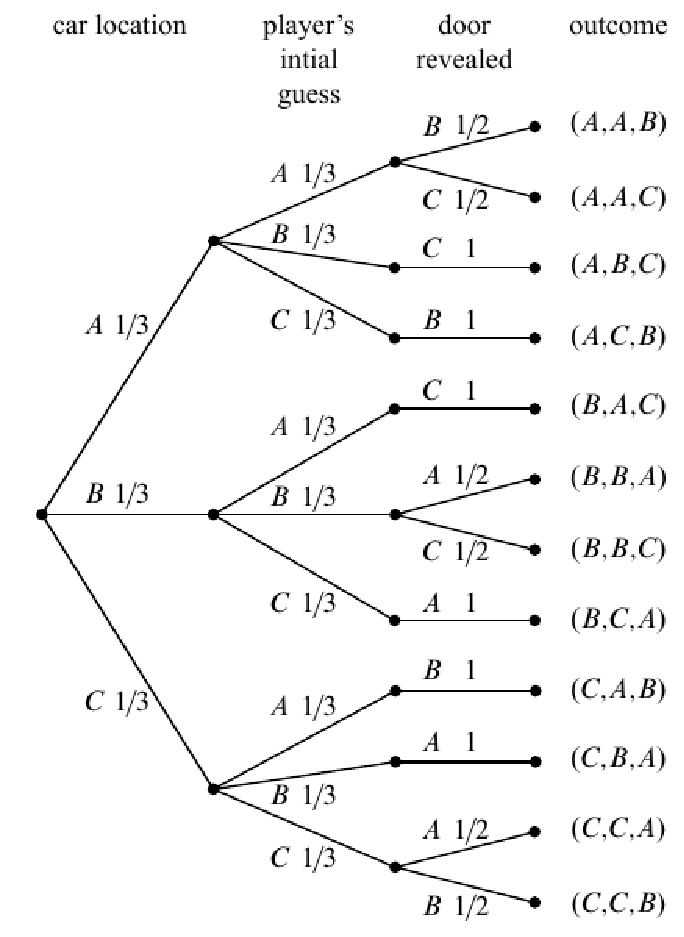
\includegraphics[scale=0.5]{fig175b.pdf}
    \end{center}
  \end{block}
\end{frame}


\begin{frame}
  \begin{dfntn}
    $$
    \pr [A \mid B] = \frac{\pr[A \cap B]}{\pr[B]}
    $$
    Nếu $\pr [B] = 0$ thì $\pr [A \mid B]$ không xác định. 
  \end{dfntn}

  \begin{xmpl}
    \begin{itemize}
    \item $F = $ sự kiện phần thưởng đặt ở cửa $A$
    \item $E = $ sự kiện người chơi chọn cửa $A$.
    \item Hỏi 
      $$
      \pr [E \cap F] = ?
      $$
    \end{itemize}
  \end{xmpl}
\end{frame}

\begin{frame}
  \begin{block}{}
    \begin{center}
      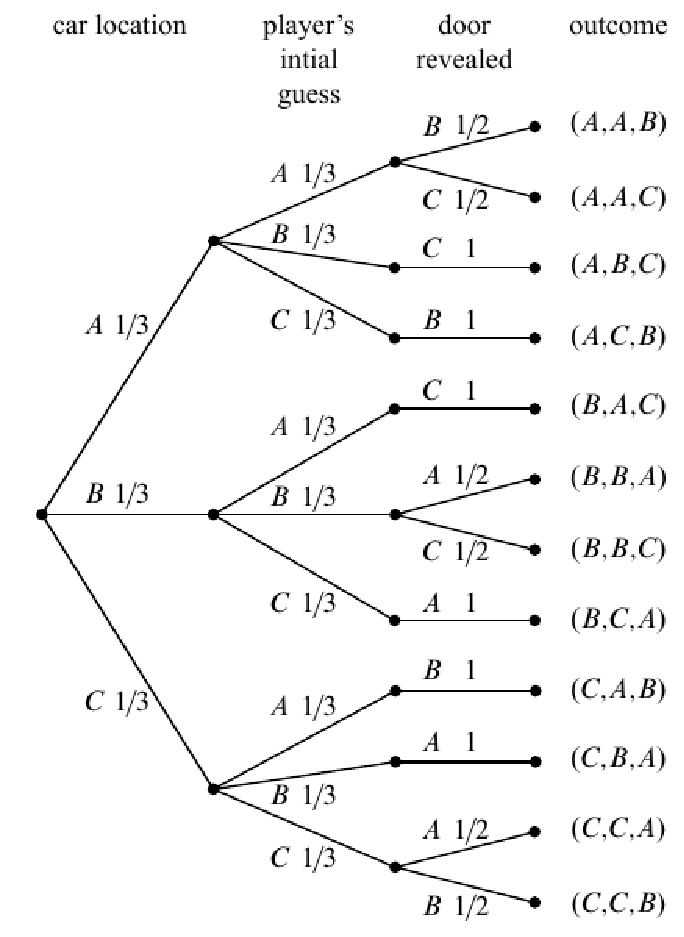
\includegraphics[scale=0.5]{fig175b.pdf}
    \end{center}
  \end{block}
\end{frame}

\begin{frame}
  \begin{xrcs}

    \begin{itemize}
    \item     Giả sử ta có hai đồng xu. 
    \item Đồng xu thật\quad  $\pr [\text{ngửa}] = \pr[\text{xấp}] = 1/2$
    \item Đồng xu giả\quad  $\pr [\text{ngửa}] = 1,\quad \pr[\text {xấp}] = 0$
    \item     Lấy một đồng với mặt ngửa lên trên, hãy  tính xác suất để đồng đó là thật.
    \end{itemize}
  \end{xrcs}
\end{frame}

\begin{frame}
  \begin{block}{Luật tích}
Nếu $\pr[B] \not = 0$, thì 
    $$\pr [A \cap B] = \pr [B]\cdot  \pr[A \mid B]$$
  \end{block}

  \begin{xmpl}
    \begin{itemize}
    \item $F = $ sự kiện phần thưởng đặt ở cửa $A$
    \item $E = $ sự kiện người chơi chọn cửa $A$.
      $$
      \pr [E \cap F] = \pr [F] \cdot \pr[E \mid F] = 1/3 \times 1/3
      $$
    \end{itemize}     
  \end{xmpl}
\end{frame}

\begin{frame}
  \begin{xrcs}
    Hãy tìm công thức cho  luật tích của  $3$ tập
    $$
    \pr [E_1 \cap E_2 \cap E_3]\ =\ ?
    $$ 
  \end{xrcs}
\end{frame}

\begin{frame}{Best-of-three playoff}
  \begin{quotation}\color{blue!70}
    A best-of-three playoff là kiểu chơi đối đầu trực tiếp giữa hai đội trong đó đội thắng hai trận sẽ thắng. Nếu một đội thắng cả hai trận đầu, trận thứ ba sẽ không phải chơi nữa.
  \end{quotation}
\begin{itemize}
  \item Xác suất đội BK thắng trận đầu là $1/2$.
  \item Với các trận sau, xác suất thắng của BK phụ thuộc vào kết quả của trận trước đó.
  \item Nếu trận trước thắng, thì trận sau cũng thắng với xác suất $2/3$.
  \item Nếu trận trước thua, thì trận sau thắng với xác suất chỉ $1/3$.
  \item Hãy tính xác suất của đội BK thắng, biết rằng họ đã thắng trận đầu tiên.
  \end{itemize}
\end{frame}

\begin{frame}
  \begin{itemize}
  \item $A = $ sự kiện đội BK thắng.
  \item $B = $ sự kiện đội BK thắng trận đầu tiên.
    $$
    \pr[A \mid B] \ = \ ?
    $$
  \end{itemize}
\end{frame}
\begin{frame}
  \begin{block}{}
    \begin{center}
      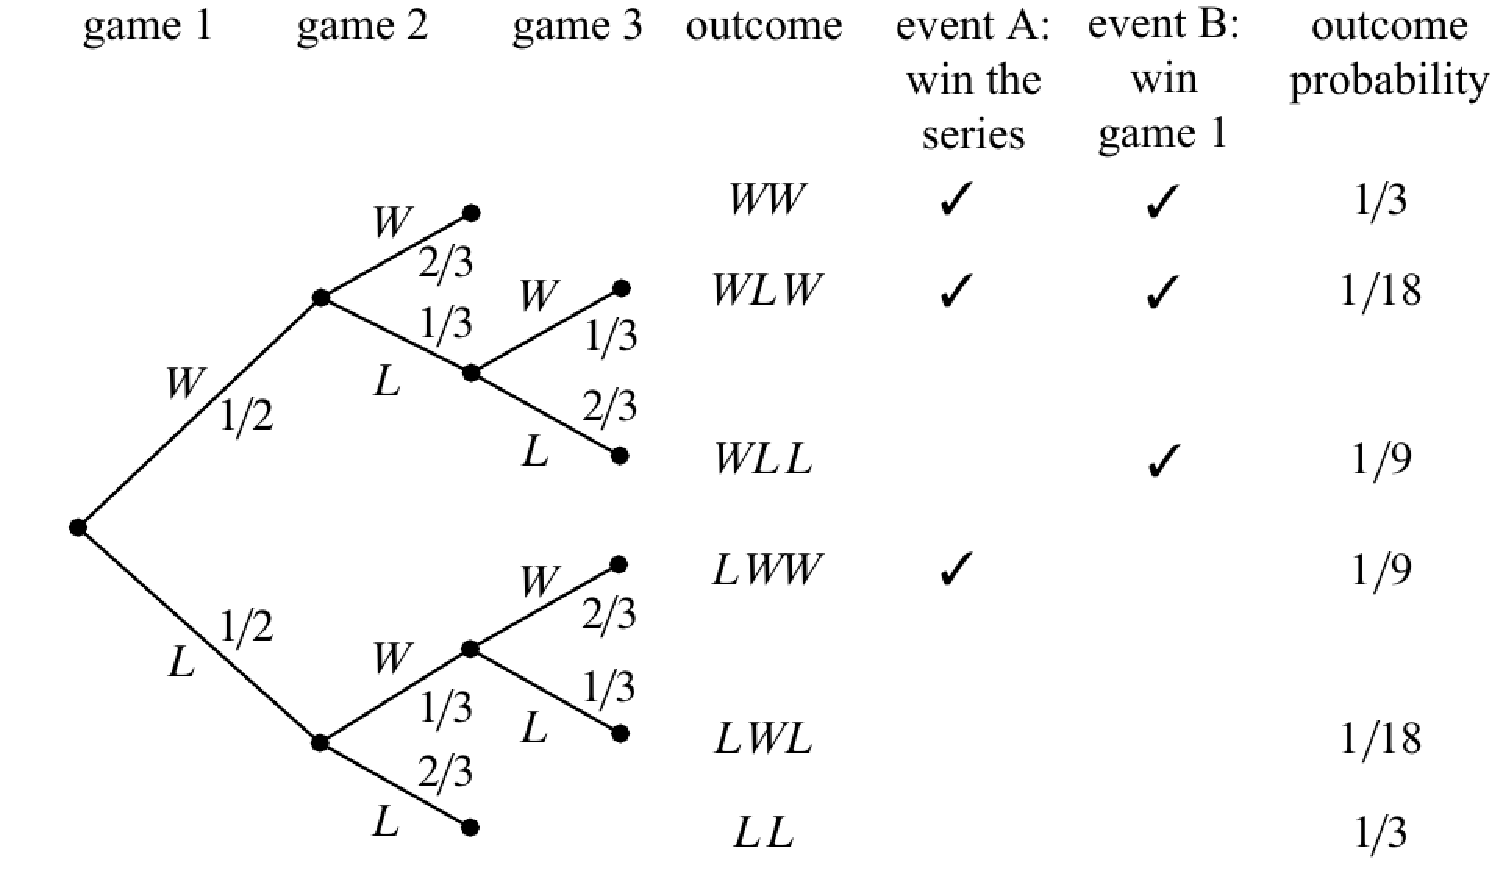
\includegraphics[width=\textwidth]{fig1713.pdf}
    \end{center}
  \end{block}
\end{frame}


  

\begin{frame}
  \begin{itemize}
  \item $A = $ sự kiện đội BK thắng.
  \item $B = $ sự kiện đội BK thắng trận đầu tiên.
    $$  
    \pr[A \mid B] = \frac{\pr[A \cap B]}{\pr[B]}\ =\ ?
    $$
    
  \end{itemize}
\end{frame}

\begin{frame}{Xác suất có điều kiện trên  cạnh của cây}
  \begin{block}{}
    \begin{center}
      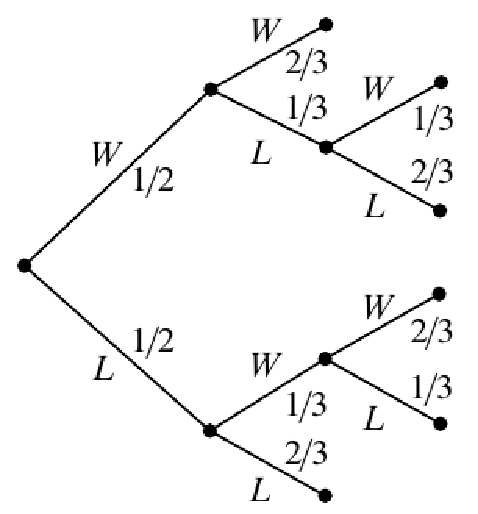
\includegraphics[width=0.4\textwidth]{fig1713b.pdf}      
    \end{center}
  \end{block}
  \begin{align*}
    \pr[WW]&=\pr[\text{thắng trận 1}]\cdot \pr[\text{thắng trận 2}\mid
    \text{thắng trận 1}] \\
           &= 1/2 \times 2/3 = 1/3
  \end{align*}
\end{frame}
% \begin{frame}
%   \begin{block}{Luật tích tổng quát}
%     $$\pr [E_1 \cap E_2 \cap \cdots \cap E_n] = \pr [E_1]\cdot  \pr[E_2 \mid E_1]\cdot \pr[E_3\mid E_1 \cap E_2]\cdots \pr[E_n\mid E_1 \cap E_2 \cap \cdots \cap E_{n-1} ]$$
%   \end{block}
% \end{frame}


\begin{frame}{Xét nghiệm y khoa}
  \begin{block}{}
    Có một bệnh mà $10\%$ dân số bị. Có một test để phát hiện bệnh tiềm ẩn; test này không phải là hoàn hảo, tuy nhiên :
    \begin{itemize}
    \item Nếu bạn có bệnh, chỉ có 10\% khả năng test nói bạn
      không có (false negatives).

    \item Nếu bạn không có bệnh, có 30\% khả năng test nói bạn có (false
      positives).
    \end{itemize}
    Giả sử một người ngẫu nhiên được test. Nếu test là  dương tính, vậy thì xác suất người này mắc bệnh là bao
    nhiêu?
  \end{block}
\end{frame}

\begin{frame}
  \begin{block}{}
    \begin{center}
      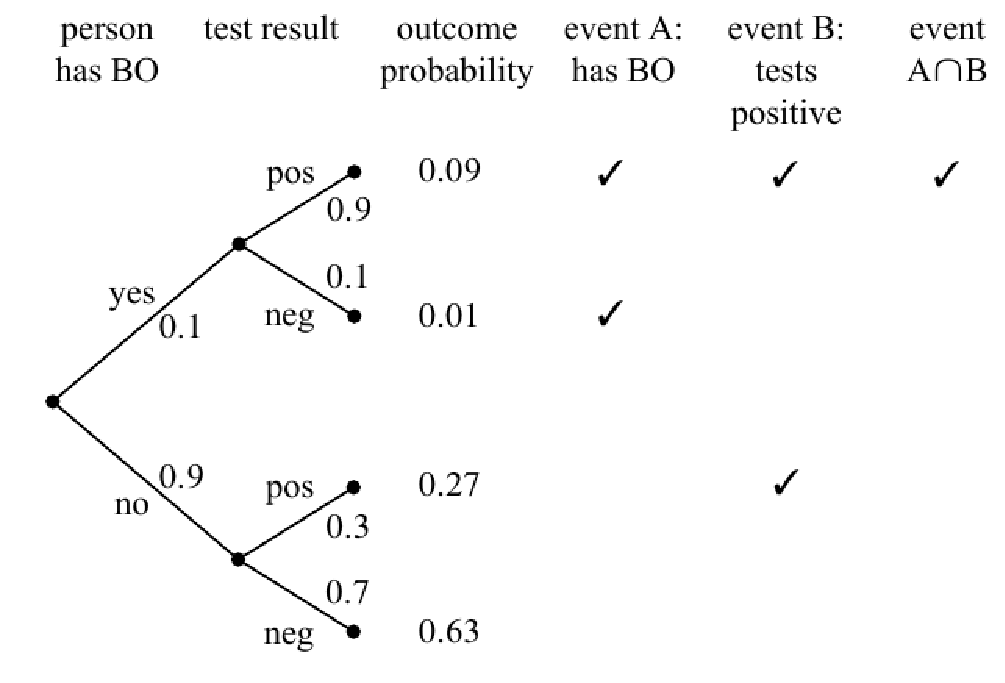
\includegraphics[width=0.9\textwidth]{fig1714.pdf}
    \end{center}
  \end{block}
\end{frame}

\begin{frame}
  \begin{itemize}
  \item $A$ sự kiện  người này  có bệnh.
  \item $B$ sự kiện người này có test dương tính.
$$  
\pr[A \mid B] = \frac{\pr[A \cap B]}{\pr[B]}\ =\ ?
$$

$$
\pr[\text{ test là đúng }]\ =\  ?
$$
  \end{itemize}
\end{frame}

\begin{frame}{Xác suất hậu nghiệm}
  \begin{xrcs}
    Trong trò chơi best-of-three, hãy tính xác suất đội BK đã thắng trận đầu tiên, biết rằng cuối cùng họ đã thắng. 
  \end{xrcs}

\end{frame}


\begin{frame}
  \begin{thrm}[Bayes]
    Nếu $\pr[A]$ và $\pr[B]$ khác $0$, vậy thì 
    $$
    \pr[B \mid A ] = \frac{\pr[A \mid B ]\cdot \pr[B]}{\pr[A]}.
    $$
  \end{thrm}
  \begin{xrcs}
    Chứng minh Định lý Bayes.
  \end{xrcs}

\end{frame}

\begin{frame}
     Đây là một bài toán được 3 nhà toán học Cassels, Shoenberger và Grayboys đem đố 60 sinh viên và cán bộ y khoa tại Harvard
Medical School năm 1978. 

  \begin{xrcs}
    \begin{itemize}
    \item Giả sử có một loại bệnh mà tỷ lệ người mắc bệnh là
      1/1000.
    \item Giả sử có một loại xét nghiệm, mà ai mắc bệnh khi xét
      cũng ra phản ứng dương tính, nhưng tỷ lệ phản ứng dương tính
      nhầm (false positive) là 5\% (tức là trong số những người không
      bị bệnh có 5\% số người thử ra phản ứng dương tính).
    \item Hỏi khi một
      người xét nghiệm bị phản ứng dương tính, thì khả năng mắc bệnh
      của người đó là bao nhiêu?
    \end{itemize}
  \end{xrcs}
\end{frame}


\end{document}


